\documentclass{article}
\usepackage[T1]{fontenc}
\usepackage{lmodern}
\usepackage{graphicx}
\usepackage{amsmath,amssymb}
\usepackage[a4paper,margin=2cm]{geometry}
\usepackage[absolute,overlay]{textpos}
\setlength{\TPHorizModule}{1mm}
\setlength{\TPVertModule}{1mm}
\usepackage[indonesian]{babel}
\usepackage{hyperref}
\setlength{\emergencystretch}{2em}
% unit: Halaman 68

\begin{document}

% === Halaman 68 (llm) ===

\vspace{270.27mm}

else
\begin{verbatim}
biner = biner(:);             % Transpose vektor biner
biner = str2num(biner);      % Ubah bit biner ke numerik

% Lakukan penyisipan bit-bit pesan ke dalam pixel-pixel
disp('Penyisipan pesan....');
idx = 1; % Mulai dari bit pertama pesan
for row = 1 : size(coverImage,1)
    for col = 1 : size(coverImage,2)
        for i = 1 : 3
            if idx <= m
                coverImage(row, col, i) = bitset(coverImage(row, col, i), 1, biner(idx));
                idx = idx + 1;
            end
        end
    end
end
stegoImage = coverImage;
% Simpan citra stego
namaFile = input('Ketikkan nama file citra stego (bmp): ', 's');
imwrite(stegoImage, namaFile);
% Tampilkan citra stego
figure; imshow(stegoImage); title ('Citra steo');
disp('Selesai');
end
\end{verbatim}

% deskripsi: Screenshot potongan kode pemrograman MATLAB untuk proses penyisipan bit pesan ke dalam citra (steganografi)
% bbox normalisasi: [0.0500, 0.0300, 0.9700, 0.9400]
\begin{textblock*}{193.20mm}(10.50mm,8.91mm)
\noindent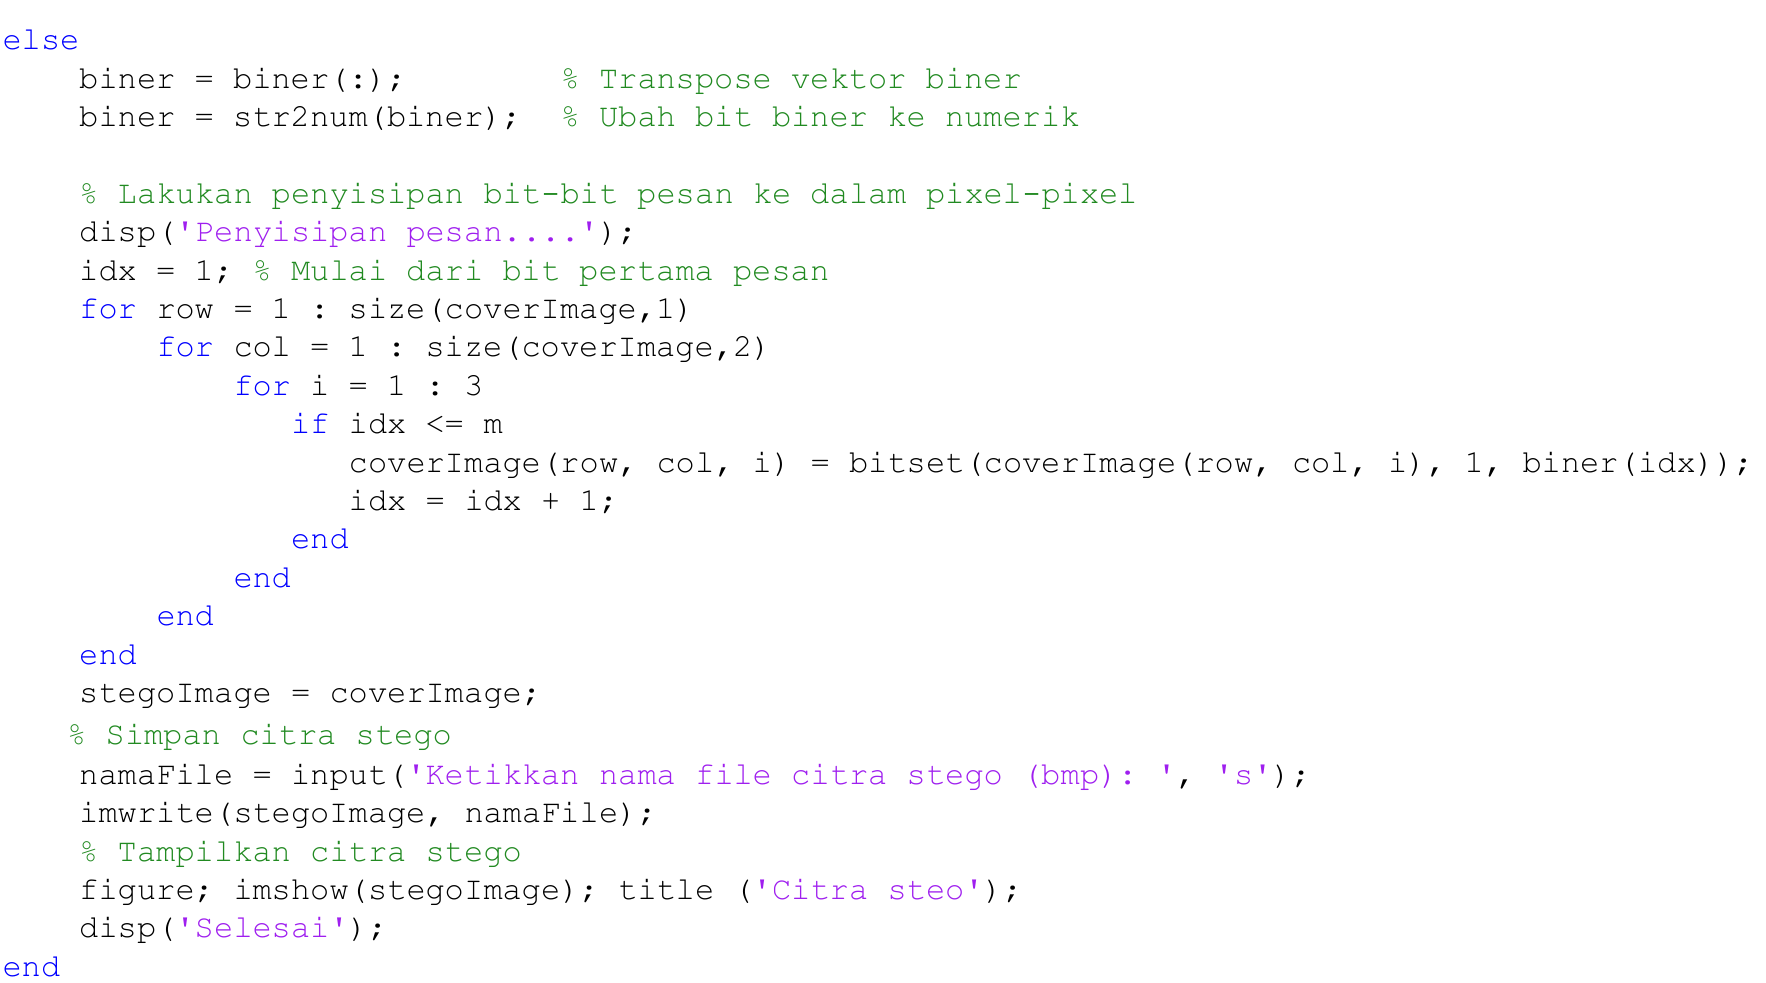
\includegraphics[width=193.20mm,height=270.27mm]{../../images/llm/page_068_img_01.png}%
\end{textblock*}

\end{document}
